% fig-convergence-triangle.tex
% "Three Traditions, One Structure"
% Standalone TikZ figure — Parts II–III
\documentclass[tikz,border=6mm]{standalone}
\usepackage{tikz}
\usepackage{xcolor}
\usetikzlibrary{arrows.meta,calc,decorations.pathmorphing,decorations.markings,shapes.geometric,positioning,backgrounds,fit,shadings,patterns}
\definecolor{substblue}{RGB}{70,130,180}
\definecolor{procamber}{RGB}{180,110,30}
\definecolor{feltgreen}{RGB}{0,110,55}
\definecolor{bgcream}{RGB}{252,248,240}
\definecolor{atomblue}{RGB}{100,160,210}
\definecolor{emphred}{RGB}{160,40,40}
\definecolor{panelborder}{RGB}{180,170,155}

\begin{document}
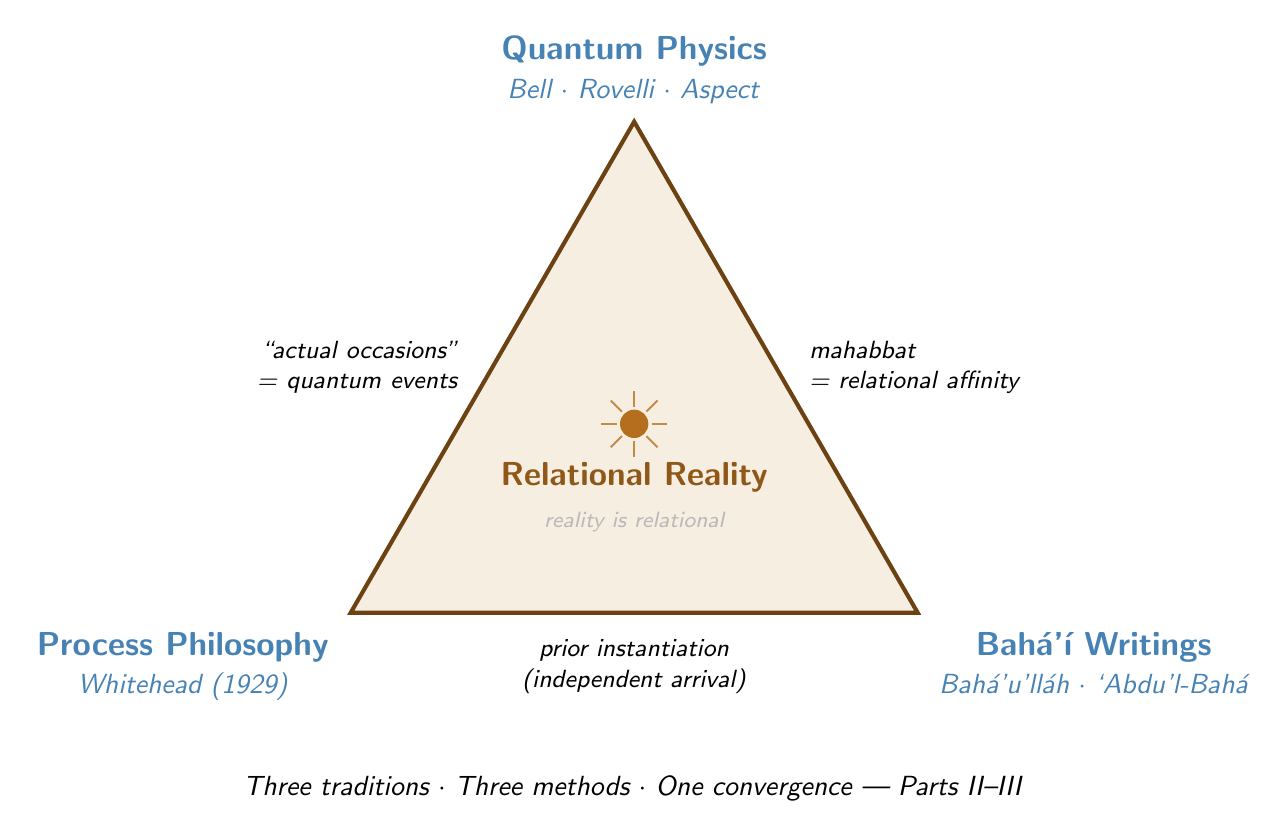
\begin{tikzpicture}[font=\sffamily]

% ── Triangle geometry ────────────────────────────────────────────────────────
% Equilateral triangle, side = 7.2 cm, centered at (6.5, 5.5)
% Top vertex, bottom-left, bottom-right
\pgfmathsetmacro{\side}{7.2}
\pgfmathsetmacro{\cx}{6.5}   % centre x
\pgfmathsetmacro{\cy}{5.5}   % centre y
\pgfmathsetmacro{\R}{\side/1.732}          % circumradius = side/√3
\pgfmathsetmacro{\r}{\side/(2*1.732)}      % inradius

% Vertices
\pgfmathsetmacro{\Tx}{\cx}
\pgfmathsetmacro{\Ty}{\cy+\R}             % top
\pgfmathsetmacro{\BLx}{\cx - \side/2}
\pgfmathsetmacro{\BLy}{\cy - \r}          % bottom-left
\pgfmathsetmacro{\BRx}{\cx + \side/2}
\pgfmathsetmacro{\BRy}{\cy - \r}          % bottom-right

% ── Triangle fill and border ─────────────────────────────────────────────────
\fill[procamber!8!bgcream!92]
  (\Tx,\Ty) -- (\BLx,\BLy) -- (\BRx,\BRy) -- cycle;
\draw[procamber!60!black, line width=1.5pt]
  (\Tx,\Ty) -- (\BLx,\BLy) -- (\BRx,\BRy) -- cycle;

% ════════════════════════════════════════════════════════════════════════════
% VERTEX LABELS
% ════════════════════════════════════════════════════════════════════════════

% TOP — Quantum Physics
\node[anchor=south, align=center, text=substblue] at (\Tx,\Ty+0.10) {
  \large\textbf{Quantum Physics}\\[2pt]
  \normalsize\textit{Bell $\cdot$ Rovelli $\cdot$ Aspect}
};

% BOTTOM-LEFT — Process Philosophy
\node[anchor=north east, align=center, text=substblue] at (\BLx-0.15,\BLy-0.12) {
  \large\textbf{Process Philosophy}\\[2pt]
  \normalsize\textit{Whitehead (1929)}
};

% BOTTOM-RIGHT — Bahá'í Writings
\node[anchor=north west, align=center, text=substblue] at (\BRx+0.15,\BRy-0.12) {
  \large\textbf{Bah\'{a}'\'{i} Writings}\\[2pt]
  \normalsize\textit{Bah\'{a}'u'll\'{a}h $\cdot$ `Abdu'l-Bah\'{a}}
};

% ════════════════════════════════════════════════════════════════════════════
% EDGE LABELS — midpoints of each side
% ════════════════════════════════════════════════════════════════════════════

% Left edge midpoint (Top ↔ Bottom-left)
\pgfmathsetmacro{\LMx}{(\Tx+\BLx)/2}
\pgfmathsetmacro{\LMy}{(\Ty+\BLy)/2}
\node[anchor=east, align=right, text width=3.0cm,
      xshift=-0.30cm] at (\LMx,\LMy) {
  \small\textit{``actual occasions''}\\[-1pt]
  \small\textit{= quantum events}
};

% Right edge midpoint (Top ↔ Bottom-right)
\pgfmathsetmacro{\RMx}{(\Tx+\BRx)/2}
\pgfmathsetmacro{\RMy}{(\Ty+\BRy)/2}
\node[anchor=west, align=left, text width=3.0cm,
      xshift=0.30cm] at (\RMx,\RMy) {
  \small\textit{\textit{mahabbat}}\\[-1pt]
  \small\textit{= relational affinity}
};

% Bottom edge midpoint (Bottom-left ↔ Bottom-right)
\pgfmathsetmacro{\BMx}{(\BLx+\BRx)/2}
\pgfmathsetmacro{\BMy}{(\BLy+\BRy)/2}
\node[anchor=north, align=center, yshift=-0.22cm] at (\BMx,\BMy) {
  \small\textit{prior instantiation}\\[-1pt]
  \small\textit{(independent arrival)}
};

% ════════════════════════════════════════════════════════════════════════════
% CENTER — Relational Reality
% ════════════════════════════════════════════════════════════════════════════
% Small filled circle / sunburst
\fill[procamber] (\cx,\cy+0.32) circle (0.18);
% Sunburst rays
\foreach \ang in {0,45,90,135,180,225,270,315}{
  \draw[procamber!80, line width=0.7pt]
    ({\cx + 0.22*cos(\ang)},{\cy+0.32 + 0.22*sin(\ang)}) --
    ({\cx + 0.42*cos(\ang)},{\cy+0.32 + 0.42*sin(\ang)});
}

\node[anchor=north, align=center] at (\cx,\cy-0.05) {
  \large\textbf{\textcolor{procamber!80!black}{Relational Reality}}\\[3pt]
  \footnotesize\textit{\textcolor{gray!55}{reality is relational}}
};

% ════════════════════════════════════════════════════════════════════════════
% CAPTION below entire figure
% ════════════════════════════════════════════════════════════════════════════
\node[anchor=north, text width=13.0cm, align=center] at (\cx,\BLy-1.95) {
  \textit{Three traditions $\cdot$ Three methods $\cdot$ One convergence --- Parts~II--III}
};

\end{tikzpicture}
\end{document}
